\documentclass[
    aspectratio=169,
    % handout
]{beamer}
% \documentclass[a4paper]{article}
% \usepackage{beamerarticle}

% Setup fonts.
\usepackage{fontspec}
\setmainfont{Iosevka Etoile}
\setsansfont{Iosevka Aile}
\setmonofont{Iosevka}


%%% Fonts and language setup.
\usepackage{polyglossia}

%% Math
\usepackage{amsmath, amsfonts, amsthm, mathtools} % Advanced math tools.
\usepackage{amssymb}

\usepackage{unicode-math} % Allow TTF and OTF fonts in math and allow direct typing unicode math characters.
\unimathsetup{
    warnings-off={
        mathtools-colon,
        mathtools-overbracket
        }
    }
% \setmathfont{Fira Math}
% \setmathfont{Noto Sans Math}[range = {\Coloneq, cal}]
% \setmathfont{Asana Math}
% [
%         Scale = MatchUppercase,
%         range = {\Coloneq, cal}
% ]
% \setmathfont{STIX Two Math}[range = {\Coloneq, cal}]
% \usepackage{euler-math}
\setmathfont{Lete Sans Math}[CharacterVariant={3,6},StylisticSet={4}]

% \usepackage{emoji}
% \setemojifont{Noto Color Emoji}

\usepackage{booktabs}
% \usepackage{colortbl}
% \usepackage{tabularx}
% \arrayrulecolor{solarizedAccent}
% \newcolumntype{Y}{>{\raggedright\arraybackslash}X}
% \newcolumntype{Z}{>{\raggedleft\arraybackslash}X}

%%% Beamer
% \usetheme{Madrid}
\usetheme{Boadilla}
% \usetheme{Berlin}
% \usecolortheme{solarized}
\usecolortheme{crane}
% \usecolortheme[style=light]{Nord}
% \usefonttheme{Nord}
\setbeamertemplate{navigation symbols}{} %remove navigation symbols
% \setbeamertemplate{headline}{%
%     \begin{beamercolorbox}[ht=2.25ex,dp=3.75ex]{section in head/foot}
%         \insertnavigation{\paperwidth}
%     \end{beamercolorbox}%
% }
\useinnertheme{circles}
\usefonttheme[stillsansserifsmall,stillsansseriftext]{serif}
% \usepackage{appendixnumberbeamer}
\setbeamertemplate{page number in head/foot}[appendixframenumber]
%% Use with Solarized theme
% \setbeamercolor{author in head/foot}{fg=solarizedRebase03}
% \setbeamercolor{title in head/foot}{fg=solarizedRebase03}
% \setbeamercolor{date in head/foot}{fg=solarizedRebase03}
% \setbeamercolor{page number in head/foot}{fg=solarizedRebase03}

%%% Misc

\setdefaultlanguage{russian}
\setotherlanguage{english}

\uselanguage{russian}
\languagepath{russian}
\newtranslation[to = russian]{Definition}{Определение}
\newtranslation[to = russian]{definition}{определение}
\newtranslation[to = russian]{Theorem}{Теорема}
\newtranslation[to = russian]{theorem}{теорема}

%% Tikz
% \usepackage{tikz}
% \usetikzlibrary{arrows.meta}
% \usetikzlibrary{external}
% \usetikzlibrary{positioning}
% \usetikzlibrary{shapes.geometric}
% \usetikzlibrary{automata}
% \usetikzlibrary{decorations.pathmorphing}
% \usetikzlibrary{calc}
% \tikzsetexternalprefix{figures/}
% \tikzexternalize

%% Pictures
\usepackage{graphicx}
\graphicspath{{figures/}}

%%% Code
\usepackage[kpsewhich,newfloat]{minted}
% \usemintedstyle{solarized-light}
\usemintedstyle{emacs}
% \SetupFloatingEnvironment{listing}{name=Листинг}

\usepackage{ebproof}

\usepackage[backend=biber, style=alphabetic]{biblatex}
\renewcommand*{\bibfont}{\footnotesize}
\addbibresource{rewriting-and-deforestation.bib}

\usepackage{csquotes}
\usepackage{hyperref}

\title[Правила переписывания и дефорестация]{Правила переписывания и немного дефорестации}
\subtitle{Функциональные техники оптимизации}
\author{Николай Пономарев}
\institute[Матмех СПбГУ]{Математико-механический факультет СПбГУ}
\date{21 декабря 2024 г.}

\begin{document}

\begin{frame}[plain, noframenumbering]
    \maketitle
\end{frame}

\begin{frame}
    \frametitle{OCaml vs. Haskell}

    % По абсолютно непонятной мне причине, при использовании \mintinline у лямбды в хаскелле пропадает пробел перед стрелочкой.
    \begin{center}
        \begin{tabular}{lcll}
            \toprule
            OCaml                             &                    & Haskell                          &                         \\
            \midrule
            \mintinline{ocaml}|f : 'a|        & $\rightsquigarrow$ & \mintinline{haskell}|f :: a|     & типовые аннотации       \\
            \mintinline{ocaml}|a :: b :: []|  & $\rightsquigarrow$ & \mintinline{haskell}|a : b : []| & Cons для списков        \\
            \mintinline{ocaml}|[1; 2; 3]|     & $\rightsquigarrow$ & \mintinline{haskell}|[1, 2, 3]|  & списки                  \\
            \mintinline{ocaml}|fun x -> body| & $\rightsquigarrow$ & \mintinline{haskell}|\x -> body| & $\lambda$-функции       \\
            \mintinline{ocaml}|'a list|       & $\rightsquigarrow$ & \mintinline{haskell}|[a]|        & Конструктор типа списка \\
            \bottomrule
        \end{tabular}
    \end{center}

\end{frame}

\begin{frame}
    \frametitle{Чистая ленивость}

    \begin{columns}[T]
        \begin{column}{0.5\textwidth}
            % https://programmerhumor.io/programming-memes/hassideeffects/
            
\includegraphics[width=0.8\linewidth, keepaspectratio]{side-effects.jpeg}
        \end{column}
        \begin{column}{0.5\textwidth}
            % https://www.reddit.com/r/ProgrammerHumor/comments/94yi0n/haskell_laziness_change_my_mind/
            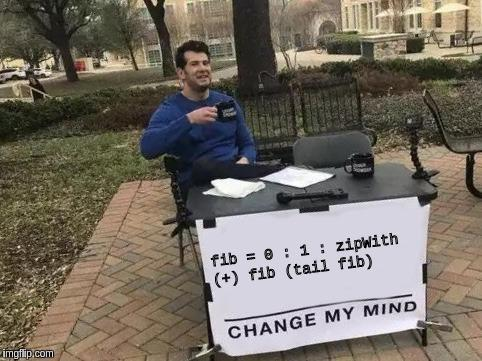
\includegraphics[width=\linewidth, keepaspectratio]{lazy.jpg}
        \end{column}
    \end{columns}

\end{frame}

\begin{frame}[fragile]
    \frametitle{Гадание на типах}

    \begin{onlyenv}<1>
        \inputminted[firstline=5, lastline=5]{haskell}{Code.hs}
    \end{onlyenv}

    \begin{onlyenv}<2>
        \inputminted[firstline=8, lastline=9]{haskell}{Code.hs}
    \end{onlyenv}

\end{frame}

\begin{frame}[fragile]
    \frametitle{Оптимальная композиция}

    \inputminted[firstline=11, lastline=13]{haskell}{Code.hs}

    \vspace{1em}

    \uncover<+->{Сколько требуется обходов списка \mintinline{haskell}|map f (map g xs)|? Промежуточных списков?}

    \uncover<+->{Обходов: 2}%
    \uncover<+->{, промежуточных списков: 1}%
    \uncover<+->{\alert{~--- плохо!}}

    \vspace{1em}
    \uncover<+->{
        Перепишем: \mintinline{haskell}|map (f . g) xs|

        Потребуется всего 1 обход и 0 промежуточных списков!
    }
\end{frame}

\begin{frame}[fragile]
    \frametitle{Можно оно само?}

    \only<+->{Хотим автоматически такое делать $\Rightarrow$ научим компилятор!}

    \begin{onlyenv}<+->
        \inputminted[firstline=15, lastline=17]{text}{Code.hs}
    \end{onlyenv}

    \vspace{1em}

    \only<+->{В GHC правила работают во всём проекте, а мейнтейнеры библиотек могут объявлять свои правила для оптимизации пользовательских функций}
\end{frame}

\begin{frame}
    \frametitle{Содержательные ограничения}

    Правила должны иметь вид \mintinline{haskell}{f e1 ... en}, при этом \texttt{f} не должна стоять под квантором

    \inputminted[firstline=112, lastline=115]{text}{Code.hs}

    \begin{itemize}
        \item Правило переписывания $\equiv$ ещё одно определение функции
        \item Упрощение поиска шаблона
        \item Не ломает другие оптимизации (inlining, let-floating, beta reduction, case swapping, case elimination, ...)
    \end{itemize}
\end{frame}

\begin{frame}[fragile]
    \frametitle{А минусы будут?}

    Система настолько проста, что опирается на адекватность автора правил

    Нет проверки на
    \begin{itemize}
        \item сохранение семантики
        \item увеличение производительности
        \item завершаемость
              \inputminted[firstline=22, lastline=23]{text}{Code.hs}
    \end{itemize}

\end{frame}

\begin{frame}[fragile]
    \frametitle{А, ой}

    \begin{itemize}
        \item В стандартной библиотеке есть медленные, зато читаемые функции
        \item Хотим ускорять ($\equiv$ переписывать) и их
        \item Просто правил переписывания не хватит
    \end{itemize}


    \begin{columns}
        \begin{column}{0.45\textwidth}
            \inputminted[firstline=25, lastline=26]{haskell}{Code.hs}
        \end{column}
        \begin{column}{0.05\textwidth}
            $\leftrightsquigarrow$
        \end{column}
        \begin{column}{0.45\textwidth}
            \inputminted[firstline=28, lastline=31]{haskell}{Code.hs}
        \end{column}
    \end{columns}
\end{frame}

\begin{frame}[fragile]
    \frametitle{Дефорестация}

    \begin{definition}[Из \cite{marlowDeforestationHigherOrderFunctions1993}]
        Deforestation is an automatic transformation scheme for functional programs which attempts to remove unnecessary intermediate data structures
    \end{definition}

    \vspace{1em}
    \begin{columns}
        \begin{column}{0.45\textwidth}
            \inputminted[firstline=33, lastline=36]{haskell}{Code.hs}
        \end{column}
        \begin{column}{0.05\textwidth}
            $\rightsquigarrow$
        \end{column}
        \begin{column}{0.45\textwidth}
            \inputminted[firstline=38, lastline=41]{haskell}{Code.hs}
        \end{column}
    \end{columns}

    \vspace{1em}
    Здравая идея, которая в своей полной мощи, оказалась слишком дорогой

\end{frame}

\begin{frame}[fragile]
    \frametitle{\texttt{foldr} всему голова}

    Оказывается, что через стандартную функцию свёртки \texttt{foldr}
    \inputminted[firstline=43, lastline=45]{haskell}{Code.hs}
    выражается множество функций работы со списками:
    \inputminted[firstline=47, lastline=51]{haskell}{Code.hs}

    \uncover<2>{\alert{Можно ли как-то сыграть на этом?}}

\end{frame}

\begin{frame}[fragile]
    \frametitle{\texttt{foldr/build} fusion}

    Заведём специальную функцию \texttt{build}
    \inputminted[firstline=53, lastline=54]{haskell}{Code.hs}
    и правило переписывания
    \inputminted[firstline=56, lastline=59]{text}{Code.hs}
\end{frame}

\begin{frame}[fragile]
    \frametitle{Умный слайд}

    \begin{theorem}[Из \cite{gillShortCutDeforestation1993} на основе \cite{wadlerTheoremsFree1989}]
        Если для некоторого фиксированного типа \texttt{A} существует

        \mintinline{haskell}{g :: forall b. (A -> b -> b) -> b -> b},

        то выполнено

        \mintinline{haskell}{foldr k z (build g) = g k z}
    \end{theorem}

\end{frame}

\begin{frame}
    \frametitle{Да зачем ты нам это всё рассказываешь?!}

    С помощью \texttt{foldr} и \texttt{build} можно ещё больше разложить функции:
    \inputminted[firstline=61, lastline=66]{haskell}{Code.hs}

    \vspace{1em}
    \uncover<2>{Вот теперь можно заняться дефорестацией!}
\end{frame}

\begin{frame}[fragile]
    \frametitle{Бесконечные списки I/II}

    \inputminted[firstline=68, lastline=76]{haskell}{Code.hs}

    Вычислим ли \texttt{x}?
    Какого его значение?

    \vspace{1em}
    \uncover<2>{\mintinline{haskell}{True}!}
\end{frame}

\begin{frame}[fragile]
    \frametitle{Бесконечные списки II/II}

    \inputminted[firstline=78, lastline=82]{haskell}{Code.hs}

\end{frame}

\begin{frame}
    \frametitle{Эффективный \texttt{all}}

    \inputminted[firstline=84, lastline=93]{haskell}{Code.hs}

\end{frame}

\begin{frame}
    \frametitle{Обобщенный Cons (Из \cite{peytonjonesPlayingRulesRewriting2001})}

    \inputminted[firstline=95, lastline=106]{haskell}{Code.hs}

\end{frame}

\begin{frame}
    \frametitle{Хотим б\'{о}льшего (по мотивам \cite{reindersHigherOrderPatterns2024})}

    Обобщим
    \inputminted[firstline=117, lastline=119]{text}{Code.hs}
    до
    \inputminted[firstline=126, lastline=129]{text}{Code.hs}
    и не сможем помэтчить \mintinline{haskell}{unzip (map (\x -> (x, x)) xs)}
\end{frame}

\begin{frame}
    \frametitle{Почему так вышло?}

    \begin{spreadlines}{2em}
        \begin{gather*}
            \begin{prooftree}
                \hypo{\text{\texttt{f}} \leftarrow \text{\texttt{g}}}
                \hypo{\text{\texttt{x}} \leftarrow \text{\texttt{y}}}
                \infer2[App]{\text{\texttt{f x}} \leftarrow \text{\texttt{g y}} }
            \end{prooftree} \qquad
            \begin{prooftree}
                \hypo{\text{\texttt{x}} \leftarrow \text{\texttt{y}}[\text{\texttt{v}} \coloneq \text{\texttt{u}}]}
                \infer1[Lam]{\text{\texttt{(\textbackslash{}u -> x)}} \leftarrow \text{\texttt{(\textbackslash{}v -> y)}}}
            \end{prooftree} \\
            \begin{prooftree}
                \infer0[Var]{\text{\texttt{v}} \leftarrow \text{\texttt{v}}}
            \end{prooftree} \qquad
            \begin{prooftree}
                \hypo{\text{\texttt{v} templ}}
                \hypo{flvs(\text{\texttt{x}}) = \varnothing}
                \infer2[Templ-Var]{\text{\texttt{v}} \leftarrow \text{\texttt{x}}}
            \end{prooftree} \\
            \begin{prooftree}
                \hypo{\text{\texttt{v} unfold to \texttt{y}}}
                \hypo{\text{\texttt{x}} \leftarrow \text{\texttt{y}}}
                \infer2[Var-Unfold]{\hypo{\text{\texttt{x}} \leftarrow \text{\texttt{v}}}}
            \end{prooftree} \qquad
            \begin{prooftree}
                \hypo{flvs(\text{\texttt{v}}) = \varnothing}
                \hypo{\text{\texttt{x}} \leftarrow \text{\texttt{z}}}
                \infer2[Let-Float]{\text{\texttt{x}} \leftarrow \text{\texttt{let v = y in z}}}
            \end{prooftree}
        \end{gather*}
    \end{spreadlines}
    % + правило для \texttt{case}
\end{frame}

\begin{frame}
    \frametitle{Пример вывода}
    \begin{scriptsize}
        \[
            \begin{prooftree}
                \infer0[Var]{\text{\texttt{map}} \leftarrow \text{\texttt{map}}}
                \infer0[Templ-Var]{\text{\texttt{f}} \leftarrow \text{\texttt{(* 2)}}}
                \infer2[App]{\text{\texttt{map f}} \leftarrow \text{\texttt{map (* 2)}}}
                \infer0[Var]{\text{\texttt{map}} \leftarrow \text{\texttt{map}}}
                \infer0[Templ-Var]{\text{\texttt{g}} \leftarrow \text{\texttt{(+ 1)}}}
                \infer2[App]{\text{\texttt{map g}} \leftarrow \text{\texttt{map (+ 1)}}}
                \infer0[Templ-Var]{\text{\texttt{xs}} \leftarrow \text{\texttt{ys}}}
                \infer2[App]{\text{\texttt{map g xs}} \leftarrow \text{\texttt{map (+ 1) ys}}}
                \infer2[App]{\text{\texttt{map f (map g xs)}} \leftarrow \text{\texttt{map (* 2) (map (+ 1) ys)}}}
            \end{prooftree}
        \]
    \end{scriptsize}

\end{frame}

\begin{frame}
    \frametitle{Чиним!}

    Интуитивно понятно, что
    \[\text{\texttt{unzip (map (\textbackslash{}x -> (f x, g x)) xs)}} \leftarrow \texttt{unzip (map (\textbackslash{}x -> (x, x)) xs)}\]
    только в случае
    $\left[\text{\texttt{f}} \coloneq (\text{\texttt{\textbackslash{}y -> y}}), \text{\texttt{g}} \coloneq (\text{\texttt{\textbackslash{}z -> z}})\right]$

    \vspace{1em}
    Добавим новое правило!
    \[
        \begin{prooftree}
            \hypo{\text{\texttt{v$_1$...v$_n$} local}\quad \text{\texttt{v$_1$...v$_n$} distinct}}
            \infer[rule style=no rule]1[]{\text{\texttt{f} templ}\quad flvs(\text{\texttt{x}}) \subseteq \{\text{\texttt{v$_1$, ..., v$_n$}}\}}
            \infer1[HOP]{\text{\texttt{f v$_1$...v$_n$}} \leftarrow \text{\texttt{x}}}
        \end{prooftree}
    \]
    Оно генерирует подстановку $\left[\text{\texttt{f}} \coloneq (\text{\texttt{\textbackslash{}v$_1$...v$_n$ -> x}})\right]$
\end{frame}

\begin{frame}
    \frametitle{Вывод с новым правилом}

    \inputminted[firstline=131, lastline=131]{text}{Code.hs}

    \[
        \begin{prooftree}
            \infer0[Var]{\text{\texttt{foo}} \leftarrow \text{\texttt{foo}}}
            \hypo{\text{\texttt{y} local}\quad \text{\texttt{y} distinct}\quad \text{\texttt{f} templ}}
            \infer[rule style=no rule]1[]{flvs(\text{\texttt{(+) ((*) y 2) y}}) = \{\text{\texttt{y}}\} \subseteq \{\text{\texttt{y}}\}}
            \infer1[HOP]{\text{\texttt{f y}} \leftarrow \text{\texttt{(+) ((*) y 2) y}}}
            \infer1[Lam]{\text{\texttt{(\textbackslash{}y -> f y)}} \leftarrow \text{\texttt{(\textbackslash{}x -> (+) ((*) x 2) x)}}}
            \infer2[App]{\text{\texttt{foo (\textbackslash{}y -> f y)}} \leftarrow \text{\texttt{foo (\textbackslash{}x -> (+) ((*) x 2) x)}}}
        \end{prooftree}
    \]
\end{frame}

\begin{frame}
    \frametitle{Stream fusion (по мотивам \cite{farmerHERMITStreamFusing2014}) I/III}

    Идея: заменить последовательность рекурсивных \enquote{трансформеров} на последовательность нерекурсивных \enquote{трансформеров}, которую завершает рекурсивный \enquote{вычислитель}

    \vspace{1em}
    \inputminted[firstline=133, lastline=136]{haskell}{Code.hs}

\end{frame}

\begin{frame}
    \frametitle{Stream fusion II/III}

    \begin{columns}[T]
        \begin{column}{0.48\textwidth}
            \inputminted[firstline=138, lastline=142]{haskell}{Code.hs}
        \end{column}
        \begin{column}{0.49\textwidth}
            \inputminted[firstline=144, lastline=149]{haskell}{Code.hs}
        \end{column}
    \end{columns}

    \inputminted[firstline=154, lastline=159]{haskell}{Code.hs}
    \inputminted[firstline=151, lastline=152]{haskell}{Code.hs}

\end{frame}

\begin{frame}
    \frametitle{Stream fusion III/III}

    Основа оптимизации~--- правило:
    \inputminted[firstline=161, lastline=161]{text}{Code.hs}

    тогда
    \inputminted[firstline=163, lastline=168]{haskell}{Code.hs}

\end{frame}

\begin{frame}
    \frametitle{А вот и не fusion}

    \inputminted[firstline=170, lastline=183]{haskell}{Code.hs}

\end{frame}

\begin{frame}
    \frametitle{Слишком сложная функция}

    \begin{displayquote}[\cite{farmerHERMITStreamFusing2014}]
        The inner stream, including its generator function, is created by applying a function to a value of the outer stream at runtime. That function could potentially pick from arbitrarily many different inner streams based on the value it is applied to. Each of these streams may have an entirely different generator function. In fact, since the type of the state in a Stream is existentially quantified, the returned streams may not even have the same state type.
    \end{displayquote}

\end{frame}

\begin{frame}
    \frametitle{Но обычно всё хорошо}

    Однако обычно вид функции не зависит от входного элемента.
    В таком случае можно использовать альтернативную функцию
    \inputminted[firstline=185, lastline=185]{haskell}{Code.hs}

    \vspace{1em}
    и правило переписывания
    \inputminted[firstline=187, lastline=190]{text}{Code.hs}

    Поскольку \texttt{next} и \texttt{f}~--- функции, то тут пригодится HOP правило
\end{frame}

\begin{frame}
    \frametitle{We're stuck!}

    \mintinline{haskell}{map (\x -> x + 1) ys} перепишется как \mintinline{haskell}{foldr (\x xs -> (x + 1) : xs) [] ys}

    \vspace{1em}
    \alert{Мы застряли!}

    \vspace{1em}
    Можно выбрать

    \begin{columns}[T]
        \begin{column}{0.49\textwidth}
            заинлайнить \mintinline{haskell}{foldr} и упростить:
            \inputminted[firstline=108, lastline=110]{haskell}{Code.hs}
        \end{column}
        \begin{column}{0.48\textwidth}
            или вернуться к

            \mintinline{haskell}{map (\x -> x + 1) ys}
        \end{column}
    \end{columns}


    \vspace{1em}
    GHC выбирает второй вариант
\end{frame}

\begin{frame}
    \frametitle{Откат переписывания}

    Без HOP выписать общее правило не получится, поэтому GHC использует функции-маркеры
    \inputminted[firstline=192, lastline=196]{text}{Code.hs}

    \vspace{1em}
    С HOP правилом можно избавиться от маркеров и напрямую заменять
    \inputminted[firstline=198, lastline=199]{text}{Code.hs}
\end{frame}

\appendix
\begin{frame}[plain, allowframebreaks]
    \frametitle{Источники}
    \printbibliography[heading=none]
\end{frame}

\begin{frame}
    \frametitle{Вопросы к экзамену}

    \begin{enumerate}
        \item Правила переписывания как способ оптимизации.
              Мотивационный пример.
              Необходимые условия корректности.
              Вид левой части правил в GHC, причины такого выбора.
              \enquote{Законы} правил переписывания в GHC.
        \item Используя foldr/build fusion устраните промежуточные структуры данных в выданной функции.
              {\footnotesize (Практическая задачка, я подразумеваю, что слайды 10 и 13 будут в доступе на экзамене.)}
        \item Постройте вывод в исчислении со слайда 19 для выданной функции и шаблона.
              {\footnotesize (Практическая задачка, я подразумеваю, что слайд 19 будет в доступе на экзамене.)}
    \end{enumerate}

\end{frame}
\end{document}
